%!TEX root = ../../Main.tex
\graphicspath{{Chapters/Hoejtalermontering/}}
%-------------------------------------------------------------------------------

\chapter{Opgaveformulering}

I denne opgave skal vi udvikle en protokol stack, som kan overføre en fil vha. den serielle port i vores virtuelle maskine. Vi bruger til øvelsen RS-232, som er en seriel digital datakommunikation. I opgaven, skal vi udvikle både en client og en server som hhv. skal stå for at sende og modtage en bestemt fil. 
Vi skal opbygge hele protokollen og derved hele laget, som en TCP-protokol. Dette indebærer linklaget, transportlaget og applikationslaget, som skal implemneteres på både client og server. Hertil skal vores link lag, gøre brug af SLIP-protokollen. Vi bruger opgave 7 som grundlag for, at lave et applikationslag, som vi kun behøver at modifisere for at kunne bruge til denne opgave. 

Vi tester først vores serielle port, for at sikre os vi har opsat porten korrekt og at vi kan skabe en forbindelse mellem de to virtuelle maskiner. 

\begin{figure}[H]
\centering
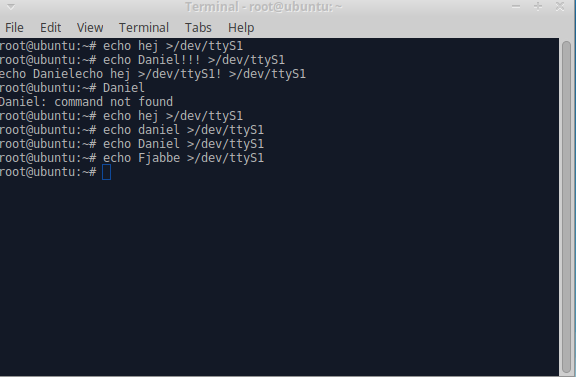
\includegraphics[width = 300 pt]{Img/opgave1.PNG}
\caption{Test vha minicom v. maskine1}
\label{fig:konceptbillede}
\end{figure}

\begin{figure}[H]
\centering
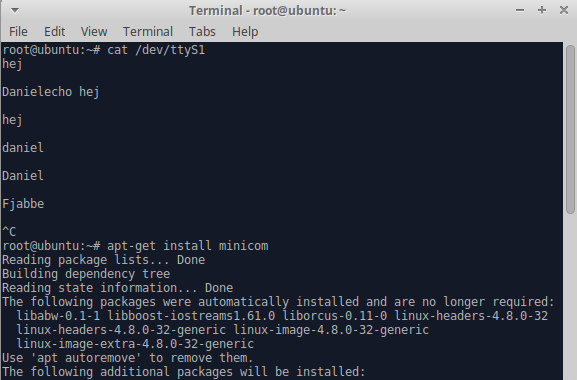
\includegraphics[width = 300 pt]{Img/opgave1_2.PNG}
\caption{Test vha minicom v. maskine2}
\label{fig:konceptbillede}
\end{figure}
    